\documentclass[9pt,aspectratio=169,xcolor=table]{beamer}

%~~~~~~~~~~~~~~~~~~~~~~~~~~~~~~~~~~~~~~~~~~~~~~~~~~~~~~~~~~~~~~~~~~~~~~~~~~~~~~
% Use roboto Font (recommended)
\usepackage[sfdefault]{roboto}
\usepackage[utf8]{inputenc}
\usepackage[T1]{fontenc}
%~~~~~~~~~~~~~~~~~~~~~~~~~~~~~~~~~~~~~~~~~~~~~~~~~~~~~~~~~~~~~~~~~~~~~~~~~~~~~~

%~~~~~~~~~~~~~~~~~~~~~~~~~~~~~~~~~~~~~~~~~~~~~~~~~~~~~~~~~~~~~~~~~~~~~~~~~~~~~~
% Define where theme files are located. ('/styles')
\usepackage{styles/fluxmacros}
\usefolder{styles}
% Use Flux theme v0.1 beta
% Available style: asphalt, blue, red, green, gray
\usetheme[style=gray]{flux}
%~~~~~~~~~~~~~~~~~~~~~~~~~~~~~~~~~~~~~~~~~~~~~~~~~~~~~~~~~~~~~~~~~~~~~~~~~~~~~~

%~~~~~~~~~~~~~~~~~~~~~~~~~~~~~~~~~~~~~~~~~~~~~~~~~~~~~~~~~~~~~~~~~~~~~~~~~~~~~~
% Extra packages
\usepackage{booktabs}
\usepackage{colortbl}
\usepackage{ragged2e}
\usepackage{amssymb}
\usepackage{multirow}
\usepackage{tikz}
\usetikzlibrary{arrows.meta, positioning, fit, backgrounds, calc, decorations.pathreplacing}
\setbeamertemplate{itemize items}[square]
\usepackage[scaled=.8]{beramono}
\usepackage{listings}
\usepackage{styles/lstlangarm}
\usepackage{array}
\definecolor{bgcolor}{HTML}{F2E9E9}
% lstlangarm.sty references \color{mauve} for string literals but never defines
% it -- only fires when a listing contains a string. Define it here.
\definecolor{mauve}{rgb}{0.58,0,0.82}
% lstlangarm's C style sets commentstyle=green!20, which is unreadable on the
% pink listing background. Darken it globally.
\lstset{commentstyle=\color{green!45!black}}
% ragged-right fixed-width column -- must be defined in the preamble, never
% inside a frame (\newcolumntype's #1 breaks beamer's frame scanner)
\newcolumntype{R}[1]{>{\RaggedRight\arraybackslash}p{#1}}
%~~~~~~~~~~~~~~~~~~~~~~~~~~~~~~~~~~~~~~~~~~~~~~~~~~~~~~~~~~~~~~~~~~~~~~~~~~~~~~
% Table striping: odd rows white, even rows very light gray.
% Needs \documentclass[...,xcolor=table]{beamer} (beamer loads xcolor itself,
% so the option must go on the class, not \usepackage).
\definecolor{stripe}{gray}{0.94}
% \striped makes body rows alternate white, gray, white, ... starting white.
% \rowcolors counts from the first coloured body row; the header is not counted.
\newcommand{\striped}{\rowcolors{1}{white}{stripe}}
%~~~~~~~~~~~~~~~~~~~~~~~~~~~~~~~~~~~~~~~~~~~~~~~~~~~~~~~~~~~~~~~~~~~~~~~~~~~~~~

%~~~~~~~~~~~~~~~~~~~~~~~~~~~~~~~~~~~~~~~~~~~~~~~~~~~~~~~~~~~~~~~~~~~~~~~~~~~~~~
% TikZ block styles -- matches ch1/ch2
% Colour variables are named identically in the book's stm32primer.tex, so any
% tikzpicture using only the \tikzset{...} styles below can be copied verbatim
% between slides and book. Only the \definecolor/\colorlet VALUES differ: the
% book is printed, so it keeps every stroke pure black with muted fills. These
% slides are projected, so both fill AND stroke are bright and saturated to
% grab attention -- see stm32primer.tex for the print palette.
\definecolor{blkfill}{HTML}{DCEBFF}
\definecolor{blkline}{HTML}{1565C0}
\definecolor{accentfill}{HTML}{FFE0B2}
\definecolor{accentline}{HTML}{E65100}
\definecolor{memfill}{HTML}{DFF5DA}
\definecolor{memline}{HTML}{2E7D32}
\definecolor{cellfill}{HTML}{FFFFFF}
\definecolor{cellline}{HTML}{424242}
\definecolor{bitmaskfill}{HTML}{DCEBFF}
\definecolor{bitmaskline}{HTML}{1565C0}
\definecolor{bithitfill}{HTML}{FFE0B2}
\definecolor{bithitline}{HTML}{E65100}
\tikzset{
  blk/.style   = {rectangle, rounded corners=2pt, draw=blkline, fill=blkfill,
                  thick, align=center, font=\small, minimum height=9mm, inner sep=3pt},
  cpublk/.style= {rectangle, rounded corners=2pt, draw=accentline, fill=accentfill,
                  thick, align=center, font=\small\bfseries, minimum height=9mm, inner sep=3pt},
  memblk/.style= {rectangle, rounded corners=2pt, draw=memline, fill=memfill,
                  thick, align=center, font=\small, minimum height=9mm, inner sep=3pt},
  cell/.style  = {rectangle, draw=cellline, fill=cellfill, align=center,
                  font=\small\ttfamily, minimum height=7mm, inner sep=2pt},
  bitcell/.style={rectangle, draw=cellline, fill=cellfill, thick,
                  minimum width=5.4mm, minimum height=5.4mm, inner sep=0pt,
                  font=\scriptsize\ttfamily, anchor=center},
  bitmask/.style={bitcell, fill=bitmaskfill, draw=bitmaskline},
  bithit/.style ={bitcell, fill=bithitfill, draw=bithitline, font=\scriptsize\ttfamily\bfseries},
  rowlab/.style ={font=\scriptsize, text=Gray, anchor=east},
  oplab/.style  ={font=\scriptsize\itshape, text=Gray, anchor=west},
  lbl/.style   = {font=\scriptsize, text=Gray},
  flow/.style  = {-{Stealth[length=2mm]}, thick, draw=blkline},
  busline/.style={thick, draw=cellline},
}
% NOTE (theme quirks -- all fail SILENTLY, always page through the PDF):
%  - a second \\ inside a nested {...} group in a TikZ node breaks parsing
%  - {\small ...} wrapped around a nested itemize eats the frame title + list
%  - \usebeamercolor on a [plain] frame falls through to an unstyled default
%  - \newcolumntype inside a frame breaks beamer's frame scanner
%  - lstlisting needs \begin{frame}[fragile]
%  - a TikZ picture wider than its column silently overflows into neighbours
%~~~~~~~~~~~~~~~~~~~~~~~~~~~~~~~~~~~~~~~~~~~~~~~~~~~~~~~~~~~~~~~~~~~~~~~~~~~~~~

%%%%%%%%%%%%%%%%%%%%%%%%%%%%%%%%%%%
%% BEGIN CONDITIONAL COMPILATION %%
%%%%%%%%%%%%%%%%%%%%%%%%%%%%%%%%%%%
\newif\ifwebex
%\webextrue % uncomment to generate section separator
\ifwebex
\AtBeginSection[]{
  \begin{frame}
  \vfill
  \centering
  \begin{beamercolorbox}[sep=8pt,center,shadow=true,rounded=true]{title}
    \usebeamerfont{title}\insertsectionhead\par%
  \end{beamercolorbox}
  \vfill
  \end{frame}
}
\else
\AtBeginSection[]
{
{
    \setbeamercolor{background canvas}{bg=yellow!10}
    \begin{frame}[plain]
        \frametitle{Table of Contents}
        \tableofcontents[currentsection]
    \end{frame}
}
}
\fi
%%%%%%%%%%%%%%%%%%%%%%%%%%%%%%%%%%%
%% END CONDITIONAL COMPILATION   %%
%%%%%%%%%%%%%%%%%%%%%%%%%%%%%%%%%%%

%~~~~~~~~~~~~~~~~~~~~~~~~~~~~~~~~~~~~~~~~~~~~~~~~~~~~~~~~~~~~~~~~~~~~~~~~~~~~~~
% Information
\title{Timers, Timing and PWM}
\subtitle{\emph{Introduction to ARM Cortex-M Microprocessors} --- Chapter 10}
\author{Mun\'{i}m Zabidi}
\institute{\color{primary}Faculty of Electrical Engineering, Universiti Teknologi Malaysia}
\date{\today}
\titlegraphic{assets/logoutmwhite.png}
%~~~~~~~~~~~~~~~~~~~~~~~~~~~~~~~~~~~~~~~~~~~~~~~~~~~~~~~~~~~~~~~~~~~~~~~~~~~~~~

\begin{document}

\titlepage

%===============================================================================
\section{Why This Matters}
%===============================================================================

\begin{frame}{Why This Chapter Matters}
    \begin{columns}[T]
    \begin{column}{.47\textwidth}
        {\normalsize \texttt{delay\_ms()} has three problems. Its timing changes with the optimizer and the clock. It uses the CPU while it waits. It gives no accurate time base. A hardware timer solves all three. It counts on its own, so it can \textbf{schedule} an event, \textbf{measure} an event, or \textbf{generate} a timed output such as PWM.}
    \end{column}
    \begin{column}{.51\textwidth}
        \begin{block}{After this chapter, you can:}
        {\small
        \begin{enumerate}\itemsep2pt
            \item Explain how prescaler and reload set a timer's period.
            \item Calculate prescaler and reload values.
            \item Generate periodic update interrupts.
            \item Keep a millisecond time base with SysTick.
            \item Choose the alternate function that routes a pin to a timer channel.
            \item Calculate PWM frequency and duty cycle.
            \item Apply PWM to LED brightness and motor speed.
        \end{enumerate}}
        \end{block}
    \end{column}
    \end{columns}
\end{frame}


%===============================================================================
\section{Why Software Delays Fail}
%===============================================================================

\begin{frame}[fragile]{Three Things Wrong With \texttt{delay\_ms()}}
    \begin{columns}[T]
    \begin{column}{.48\textwidth}
\begin{lstlisting}[style=myc]
	void delay_ms(int n) {
		for (volatile int i = 0;
		i < n * 4000; i++) ;
	}
\end{lstlisting}
    \end{column}
    \begin{column}{.48\textwidth}
        \begin{enumerate}
            \item Its timing changes with the \alert{compiler optimisation
                  level} and the \alert{clock frequency}
            \item It consumes \alert{100\%} of the CPU while waiting
            \item It cannot be \alert{interrupted accurately} --- any ISR that
                  fires makes the delay longer
        \end{enumerate}
    \end{column}
    \end{columns}

    \vspace{3mm}
    \begin{block}{A timer is a counter in hardware}
        It runs independently of the processor, at a rate you configure. It does
        not care what the CPU is doing, what the optimiser did, or how many
        interrupts fired. \alert{That is what makes it a clock rather than a
        guess.}
    \end{block}
\end{frame}

%===============================================================================
\section{Timer Architecture}
%===============================================================================

\begin{frame}{Prescaler and Auto-Reload}
    \begin{center}
    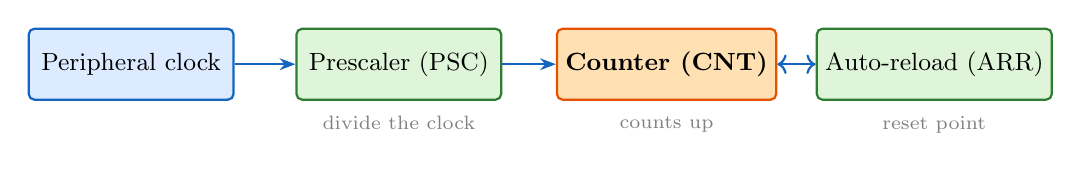
\begin{tikzpicture}[x=10mm, y=9mm]
        \node[blk,    minimum width=26mm] (clk) at (0,0)   {Peripheral clock};
        \node[memblk, minimum width=26mm] (psc) at (3.4,0) {Prescaler (PSC)};
        \node[cpublk, minimum width=26mm] (cnt) at (6.8,0) {Counter (CNT)};
        \node[memblk, minimum width=26mm] (arr) at (10.2,0){Auto-reload (ARR)};
        \draw[flow] (clk) -- (psc);
        \draw[flow] (psc) -- (cnt);
        \draw[flow, <->] (cnt) -- (arr);
        \node[lbl, anchor=north, align=center] at (3.4,-0.6) {divide the clock};
        \node[lbl, anchor=north, align=center] at (6.8,-0.6) {counts up};
        \node[lbl, anchor=north, align=center] at (10.2,-0.6) {reset point};
    \end{tikzpicture}
    \end{center}

    \vspace{3mm}
    \begin{center}
    \fbox{\parbox{.82\textwidth}{\centering\vspace{1mm}
    $f_{\text{event}} = \dfrac{f_{\text{CK}}}{(\text{PSC} + 1) \times (\text{ARR} + 1)}$
    \vspace{1mm}}}
    \end{center}

    \vspace{3mm}
    {\small The \alert{$+1$} is because a value of 0 means ``divide by 1'' --- a
    counter that reloads at 0 still counts one tick.}
\end{frame}

\begin{frame}{A Timing Calculation}
    \begin{columns}[T]
    \begin{column}{.46\textwidth}
        \textbf{Required}

        \vspace{1mm}
        {\small A 1\,Hz interrupt from a 16\,MHz clock.}

        \vspace{3mm}
        \textbf{Choose a prescaler}

        \vspace{1mm}
        {\small $\text{PSC} = 15999$ divides 16\,MHz down to
        \alert{1\,kHz} --- a convenient 1\,ms tick.}
    \end{column}
    \begin{column}{.5\textwidth}
        \textbf{Then the reload value}

        \vspace{1mm}
        {\small $\text{ARR} = 999$ gives 1000 ticks $=$ \alert{1\,s}.}

        \vspace{3mm}
        {\small Check:
        $\dfrac{16{,}000{,}000}{16000 \times 1000} = 1$\,Hz.}

        \vspace{3mm}
        {\ttfamily\scriptsize
        TIM2->PSC = 15999; \\
        TIM2->ARR = 999;}
    \end{column}
    \end{columns}

    \vspace{3mm}
    \begin{block}{Why choose PSC first}
        Both registers are 16-bit, so neither can exceed 65535. Pick the
        prescaler to give a \alert{convenient tick} --- 1\,ms or 1\,\textmu s ---
        then the reload value is just the number of ticks you want.
    \end{block}
\end{frame}

\begin{frame}[fragile]{A Periodic Timer Interrupt}
\begin{lstlisting}[style=myc, basicstyle=\ttfamily\small]
RCC->APB1ENR |= (1U << 0);      // TIM2 clock
TIM2->PSC = 15999;              // 16 MHz -> 1 kHz
TIM2->ARR = 999;                // 1000 ticks -> 1 Hz
TIM2->DIER |= (1U << 0);        // update interrupt enable
TIM2->CR1  |= (1U << 0);        // start counting
NVIC_EnableIRQ(TIM2_IRQn);

void TIM2_IRQHandler(void)
{
    if (TIM2->SR & (1U << 0)) { // update flag?
        TIM2->SR &= ~(1U << 0); // clear it
        GPIOA->ODR ^= (1U << 5);
    }
}
\end{lstlisting}

    \vspace{2mm}
    {\small The CPU is now \alert{free} between interrupts --- it can sleep, or do
    real work, and the LED still blinks at exactly 1\,Hz.}
\end{frame}

\begin{frame}[fragile]{SysTick}{The system time base}
    \begin{columns}[T]
    \begin{column}{.5\textwidth}
        \begin{itemize}
            \item A \alert{24-bit} down-counter built into the \alert{core}, not
                  the vendor's peripherals.
            \item Present on \alert{every} Cortex-M, at the same address --- so
                  code using it is portable.
            \item Normally configured for a \alert{1\,ms} tick.
        \end{itemize}

        \vspace{2mm}
        {\ttfamily\scriptsize SysTick\_Config(SystemCoreClock / 1000);}
    \end{column}
    \begin{column}{.46\textwidth}
\begin{lstlisting}[style=myc, basicstyle=\ttfamily\small]
	volatile uint32_t ticks = 0;

	void SysTick_Handler(void)
	{
		ticks++;
	}

	uint32_t millis(void)
	{
		return ticks;
	}
\end{lstlisting}
    \end{column}
    \end{columns}

    \vspace{3mm}
    \begin{block}{This is what replaces \texttt{delay\_ms()}}
        Instead of \emph{waiting}, record when something last happened and check
        whether enough time has passed. That is the \alert{non-blocking} pattern
        Chapter 14 builds a whole system from.
    \end{block}
\end{frame}


\begin{frame}[fragile]{The Bad \texttt{delay\_ms()} --- For Comparison}
\begin{lstlisting}[style=myc, basicstyle=\ttfamily\small]
		void delay_ms_bad(int n)
		{
			for (volatile int i = 0; i < n * 4000; i++)
			;
			/* Wrong in three ways: drifts with optimisation level
			and clock frequency, burns 100% CPU, and any ISR that
			fires makes it longer than requested. Do not use this
			in real designs. */
		}
	\end{lstlisting}
\end{frame}

\begin{frame}[fragile]{A Proper \texttt{delay\_ms()} --- Built on SysTick}
\begin{lstlisting}[style=myc, basicstyle=\ttfamily\small]
		static volatile uint32_t systick_ms = 0;

		void SysTick_Handler(void) { systick_ms++; }

		void systick_init(uint32_t core_clock_hz)
		{
			SysTick_Config(core_clock_hz / 1000U); // 1 ms tick
		}

		uint32_t millis(void) { return systick_ms; }

		// Blocking, but exact regardless of compiler optimisation:
		// it counts real elapsed ticks, not a fixed loop count.
		void delay_ms(uint32_t n)
		{
			uint32_t start = millis();
			while ((millis() - start) < n) {
				__asm volatile ("wfi");  // sleep between ticks
			}
		}
	\end{lstlisting}
\end{frame}

\begin{frame}[fragile]{An Alternative: \texttt{delay\_ms()} on a General-Purpose Timer}
\begin{lstlisting}[style=myc, basicstyle=\ttfamily\small]
		void tim2_delay_init(void)
		{
			RCC->APB1ENR |= (1U << 0);  // TIM2 clock enable
			TIM2->PSC = 15999;          // 16 MHz -> 1 kHz
			TIM2->ARR = 0xFFFF;         // free-running
			TIM2->CR1 |= (1U << 0);     // start counting
		}

		void delay_ms_tim2(uint32_t n)
		{
			TIM2->CNT = 0;
			while (TIM2->CNT < n)
			;
		}
	\end{lstlisting}
	{\small Useful when SysTick is already claimed by an RTOS, and the
		mechanism is the same prescaler/auto-reload arithmetic from earlier in
		this chapter.}
\end{frame}


%===============================================================================
\section{Alternate Functions}
%===============================================================================

\begin{frame}[plain]{Routing a Pin to a Peripheral}
    \begin{center}
    \includegraphics[width=.88\textwidth, height=.6\textheight, keepaspectratio]%
        {assets/afr-mux.pdf}
    \end{center}

    \vspace{2mm}
    {\small\centering A pin can serve several peripherals. \texttt{MODER} set to
    \alert{\texttt{10}} selects alternate-function mode; \texttt{AFR} then chooses
    \alert{which} of up to sixteen functions.\par}
\end{frame}

\begin{frame}[fragile]{Selecting the Function Number}
    \begin{center}
    \includegraphics[width=.9\textwidth, height=.40\textheight, keepaspectratio]%
        {assets/afrl-bits.pdf}
    \end{center}

    \vspace{2mm}
    \begin{columns}[T]
    \begin{column}{.5\textwidth}
        {\small \alert{Four bits per pin}, so \texttt{AFR[0]} covers pins 0--7 and
        \texttt{AFR[1]} covers pins 8--15.}

        \vspace{2mm}
        {\small For pin $n \geq 8$ the shift is $(n - 8) \times 4$.}
    \end{column}
    \begin{column}{.46\textwidth}
\begin{lstlisting}[style=myc, basicstyle=\ttfamily\small]
// PA5 -> TIM2_CH1 is AF1
GPIOA->MODER &= ~(3U << 10);
GPIOA->MODER |=  (2U << 10);

GPIOA->AFR[0] |= (1U << (5*4));
\end{lstlisting}
    \end{column}
    \end{columns}

    \vspace{2mm}
    {\small The function numbers are in the \alert{datasheet}, not the reference
    manual --- a distinction that costs people an afternoon.}
\end{frame}

%===============================================================================
\section{PWM}
%===============================================================================

\begin{frame}{Pulse Width Modulation}
    \begin{center}
    \begin{tikzpicture}[x=10mm, y=7mm]
        \draw[busline, thick] (0,0) -- (0,1) -- (1.5,1) -- (1.5,0) -- (3,0)
                              -- (3,1) -- (4.5,1) -- (4.5,0) -- (6,0)
                              -- (6,1) -- (7.5,1) -- (7.5,0) -- (8.5,0);
        \draw[<->, draw=primary] (0,-0.6) -- (3,-0.6);
        \node[lbl, anchor=north, text=primary] at (1.5,-0.65) {period $T$};
        \draw[<->, draw=secondary] (0,1.5) -- (1.5,1.5);
        \node[lbl, anchor=south, text=secondary] at (0.75,1.55) {on-time};
    \end{tikzpicture}
    \end{center}

    \vspace{3mm}
    \begin{center}
    \fbox{\parbox{.7\textwidth}{\centering\vspace{1mm}
    duty cycle $=\dfrac{\text{on-time}}{T}$ \qquad
    $f_{\text{PWM}} = \dfrac{f_{\text{CK}}}{(\text{PSC}+1)(\text{ARR}+1)}$
    \vspace{1mm}}}
    \end{center}

    \vspace{3mm}
    \begin{block}{A digital pin producing an analog effect}
        The pin is only ever fully on or fully off --- but switch it fast enough
        and an LED looks \alert{dimmed}, a motor runs \alert{slower}, a heater
        delivers \alert{less power}. The average is what the load responds to.
    \end{block}
\end{frame}



\begin{frame}[fragile]{Configuring PWM}

\begin{lstlisting}[style=myc, basicstyle=\ttfamily\small]
TIM2->PSC  = 15;                 // 16 MHz -> 1 MHz
TIM2->ARR  = 999;                // 1 MHz / 1000 = 1 kHz PWM
TIM2->CCR1 = 250;                // 250/1000 = 25% duty

TIM2->CCMR1 |= (6U << 4);        // PWM mode 1 on channel 1
TIM2->CCMR1 |= (1U << 3);        // preload enable
TIM2->CCER  |= (1U << 0);        // enable the output
TIM2->CR1   |= (1U << 0);        // start
\end{lstlisting}

    \vspace{2mm}
    \begin{block}{\texttt{ARR} sets the frequency, \texttt{CCR} sets the duty}
        Change \texttt{CCR1} at any time and the duty cycle changes on the next
        cycle --- no glitch, because the preload register updates only at the
        reload point. \alert{That is what makes smooth dimming possible.}
    \end{block}

    \vspace{1mm}
    {\small A higher PWM frequency is less visible but wastes more switching
    energy. For LEDs, 1\,kHz is comfortably above flicker perception.}
\end{frame}


\begin{frame}[fragile]{PWM Duty-Cycle Helper}
\begin{lstlisting}[style=myc, basicstyle=\ttfamily\small]
		void pwm_init_tim2_ch1(uint32_t psc, uint32_t arr)
		{
			RCC->APB1ENR |= (1U << 0);
			TIM2->PSC = psc;
			TIM2->ARR = arr;
			TIM2->CCR1 = 0;                // start at 0% duty
			TIM2->CCMR1 |= (6U << 4);      // PWM mode 1, channel 1
			TIM2->CCMR1 |= (1U << 3);      // preload enable
			TIM2->CCER  |= (1U << 0);      // enable output
			TIM2->CR1   |= (1U << 0);      // start
		}

		// percent: 0-100
		void pwm_set_duty_percent(uint8_t percent)
		{
			if (percent > 100) percent = 100;
			uint32_t arr = TIM2->ARR;
			TIM2->CCR1 = ((uint32_t)percent * (arr + 1)) / 100U;
		}
	\end{lstlisting}
\end{frame}

\begin{frame}[fragile]{Example: A Breathing LED, Non-Blocking}
\begin{lstlisting}[style=myc, basicstyle=\ttfamily\small]
		void led_breathe_demo(void)
		{
			static periodic_task_t step = { .last_ms = 0, .period_ms = 20 };
			static int duty = 0;
			static int dir  = 1;

			if (task_due(&step)) {
				duty += dir;
				if (duty >= 100 || duty <= 0) dir = -dir;
				pwm_set_duty_percent((uint8_t)duty);
			}
		}
	\end{lstlisting}
	{\small Every 20\,ms the duty cycle steps by one percentage point up or
		down, driven entirely by \texttt{task\_due()} --- no blocking call
		anywhere in the loop.}
\end{frame}

\begin{frame}{LED Brightness Control with PWM}
	\centering
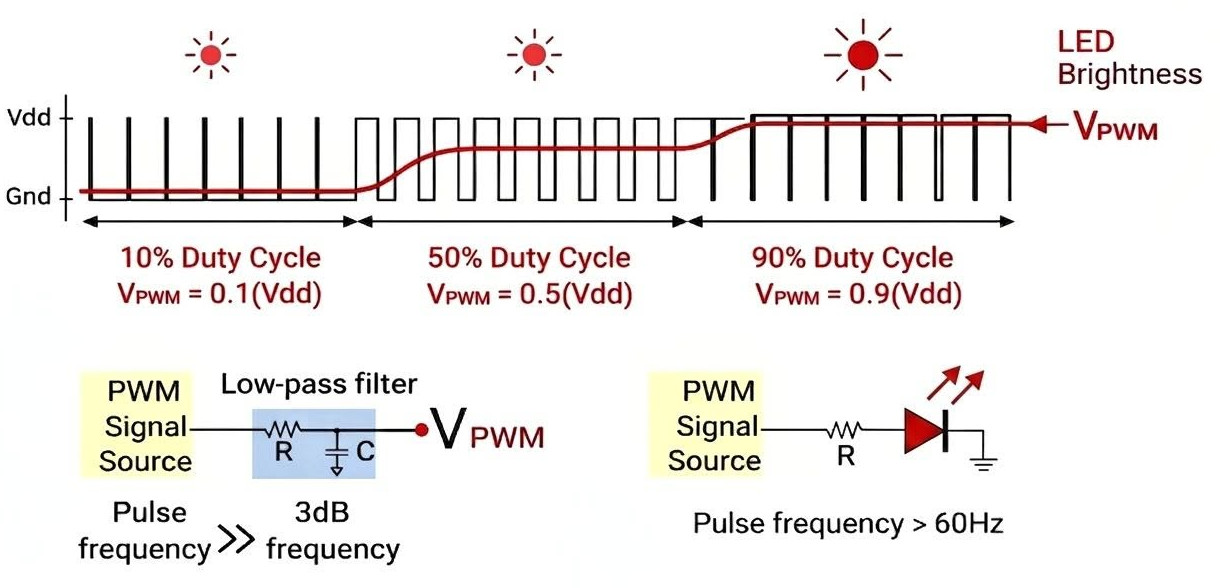
\includegraphics[width=0.92\textwidth]{assets/led_control_pwm.jpg}
\end{frame}

\begin{frame}{One PWM Output, Three Applications}
    \begin{center}
    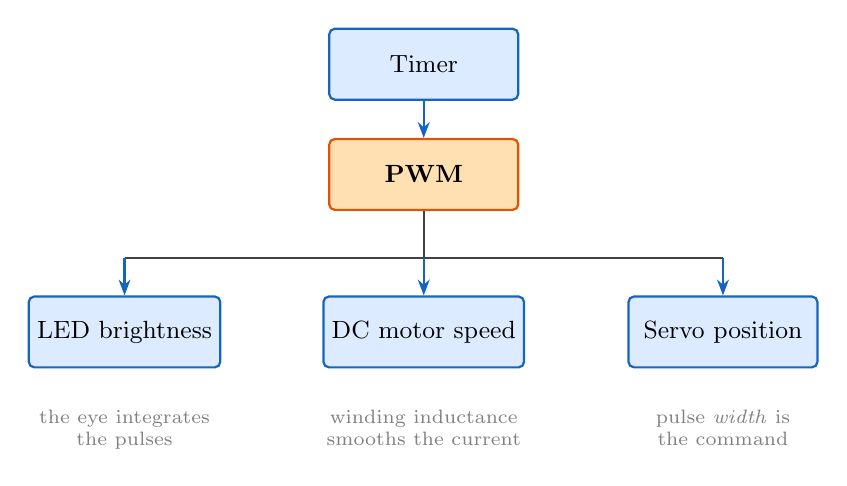
\begin{tikzpicture}[x=10mm, y=10mm]
        \node[blk, minimum width=24mm] (timer) at (0,2.4) {Timer};
        \node[cpublk, minimum width=24mm] (pwm) at (0,1.0) {PWM};
        \node[blk, minimum width=24mm] (led)   at (-3.8,-1.0) {LED brightness};
        \node[blk, minimum width=24mm] (motor) at ( 0.0,-1.0) {DC motor speed};
        \node[blk, minimum width=24mm] (servo) at ( 3.8,-1.0) {Servo position};
        \draw[flow] (timer) -- (pwm);
        \coordinate (fan) at ($(pwm.south)+(0,-0.6)$);
        \draw[busline] (pwm.south) -- (fan);
        \draw[busline] (led.north |- fan) -- (servo.north |- fan);
        \foreach \p in {led,motor,servo}{\draw[flow] (\p.north |- fan) -- (\p.north);}
        \node[lbl, below=4mm of led,   align=center] {the eye integrates\\the pulses};
        \node[lbl, below=4mm of motor, align=center] {winding inductance\\smooths the current};
        \node[lbl, below=4mm of servo, align=center] {pulse \emph{width} is\\the command};
    \end{tikzpicture}
    \end{center}

    \vspace{2mm}
    {\small LED and motor rely on \alert{physical averaging}. A servo is
    different: its control electronics measure the \alert{pulse width}
    and use it to set a position.}
\end{frame}

\begin{frame}{PWM Output at Five Levels}
    \begin{center}
    {\small
    \striped
    \begin{tabular}{@{}l R{.65\textwidth}@{}}
        \toprule
        \textbf{Level} & \textbf{Representation} \\
        \midrule
        Physical hardware & Counter, comparator and output flip-flop driving the pad \\
        Register          & \texttt{TIM2\_CCR1} compared against \texttt{TIM2\_CNT} \\
        C                 & \texttt{TIM2->CCR1 = 500;} \\
        Assembly          & \texttt{MOV R0, \#500} / \texttt{STR R0, [R1, \#0x34]} \\
        Observable        & A 1~kHz square wave at 50\% duty on pin PA5 \\
        \bottomrule
    \end{tabular}}
    \end{center}

    \vspace{3mm}
    \begin{block}{So far}
        \texttt{ARR} determines the PWM \alert{period}. \texttt{CCRx}
        determines how long the output stays \alert{high}. The same two
        registers used earlier to schedule an interrupt now generate a
        waveform instead.
    \end{block}
\end{frame}

\begin{frame}{Summary}
	\begin{columns}[c]
		\begin{column}{.62\textwidth}
			\begin{center}
				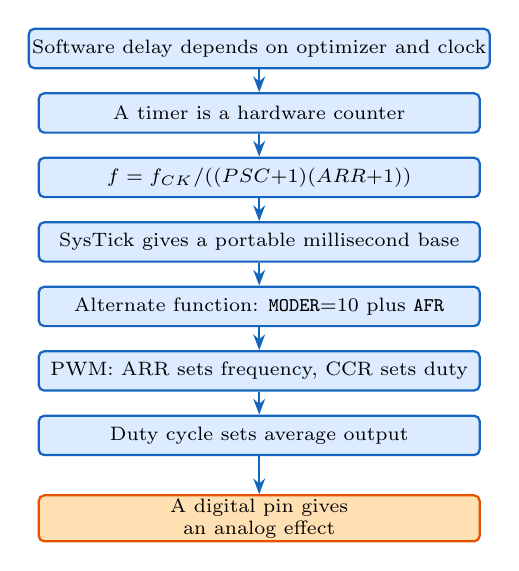
\begin{tikzpicture}[x=10mm, y=7.8mm]
					\node[blk, minimum width=56mm, minimum height=5.0mm, inner sep=1.2pt, font=\scriptsize] (n0) at (0,0.00) {Software delay depends on optimizer and clock};
					\node[blk, minimum width=56mm, minimum height=5.0mm, inner sep=1.2pt, font=\scriptsize] (n1) at (0,-1.05) {A timer is a hardware counter};
					\node[blk, minimum width=56mm, minimum height=5.0mm, inner sep=1.2pt, font=\scriptsize] (n2) at (0,-2.10) {$f = f_{\text{CK}}/((\text{PSC}{+}1)(\text{ARR}{+}1))$};
					\node[blk, minimum width=56mm, minimum height=5.0mm, inner sep=1.2pt, font=\scriptsize] (n3) at (0,-3.15) {SysTick gives a portable millisecond base};
					\node[blk, minimum width=56mm, minimum height=5.0mm, inner sep=1.2pt, font=\scriptsize] (n4) at (0,-4.20) {Alternate function: \texttt{MODER}=10 plus \texttt{AFR}};
					\node[blk, minimum width=56mm, minimum height=5.0mm, inner sep=1.2pt, font=\scriptsize] (n5) at (0,-5.25) {PWM: ARR sets frequency, CCR sets duty};
					\node[blk, minimum width=56mm, minimum height=5.0mm, inner sep=1.2pt, font=\scriptsize] (n6) at (0,-6.30) {Duty cycle sets average output};
					\node[cpublk, minimum width=56mm, minimum height=5.0mm, inner sep=1.2pt, font=\scriptsize, align=center] (n7) at (0,-7.65) {A digital pin gives\\an analog effect};
					\foreach \a/\b in {0/1,1/2,2/3,3/4,4/5,5/6,6/7}{\draw[flow] (n\a) -- (n\b);}
				\end{tikzpicture}
			\end{center}
		\end{column}
		\begin{column}{.34\textwidth}
			{\scriptsize
				\textbf{Terminology covered}\\[1mm]
				\begin{itemize}
					\item Prescaler (PSC), reload (ARR)
					\item SysTick
					\item Alternate function, \texttt{AFR}
					\item PWM, duty cycle, \texttt{CCR}
				\end{itemize}
				\vspace{3mm}
				\textbf{Next: Chapter 11}\\[1mm]
				\emph{ADC and Analog Interfacing}\\[1mm]
				We made an analog effect. Next, we measure a real one.}
		\end{column}
	\end{columns}
\end{frame}

\end{document}

